\documentclass[notes]{subfiles}
\begin{document}
	\addcontentsline{toc}{section}{2.3 - Rates of Change: Notation \& Interpretation}
	\refstepcounter{section}
	\fancyhead[RO,LE]{\bfseries  \large \nameref{cs23}} 
	\fancyhead[LO,RE]{\bfseries  \currentname}
	\fancyfoot[C]{{}}
	\fancyfoot[RO,LE]{\large \thepage}	%Footer on Right \thepage is pagenumber
	\fancyfoot[LO,RE]{\large Chapter 2.3}


\section*{Rates of Change: Notation \& Interpretation}\label{cs23}
	\subsection*{Average ROC vs. Instantaneous ROC}
		\textbf{Average Rate of Change}\showto{st}{\\[5pt]}
			\begin{itemize}
				\item \showto{ins}{\fbox{Measures how rapidly a quantity changes \emph{over an interval}.}}\showto{st}{\blank{6}\\[10pt]}
				\item \showto{ins}{\fbox{Slope of the secant line between two points.}}\showto{st}{\blank{6}}
			\end{itemize}
			\vs{1}
		\textbf{(Instantaneous) Rate of Change}\showto{st}{\\[5pt]}
			\begin{itemize}
				\item \showto{ins}{\fbox{Measures how rapidly a quantity is changing at \emph{a specific point}.}}\showto{st}{\blank{6}\\[10pt]}
				\item \showto{ins}{\fbox{Slope of the tangent line at a single point.}}\showto{st}{\blank{6}\\[10pt]}
				\item \showto{ins}{\fbox{Function must be smooth and continuous.}}\showto{st}{\blank{6}}
			\end{itemize}
			\vs{1}
			
	\subsection*{Notation and Terminology}
		Rate of change at a specific point $a$ is often referred to as any of the following (given a function $f$):\\
			\begin{itemize}
				\item \showto{ins}{\fbox{the derivative of $f$ at $a$}}\showto{st}{\blank{6}\\}
				\item \showto{ins}{\fbox{the slope of a graph of $f$ at point $(a,f(a))$}}\showto{st}{\blank{6}\\}
				\item \showto{ins}{\fbox{the slope of the line tangent to a graph of $f$ at a point $(a,f(a))$}}\showto{st}{\blank{6}\\}
				\item \showto{ins}{\fbox{the rate of change of $f$ at $a$}}\showto{st}{\blank{6}}
			\end{itemize}
				\vs{1}
		We also have two different notations for the derivative of $f$ at point $a$:
			\begin{itemize}
				\item $f'(a)$.  This is read ``$f$ prime of $a$''.
				\item $\dfrac{df}{dx}\bigg|_{x = a}$.  This is read ``d-f d-x, evaluated at $a$'', or as ``the derivative of $f$ with respect to $x$,\\[5pt] evaluated at $a$''.
			\end{itemize}
				\vs{1}
				
			\textsc{Note}: We will freely interchange between \emph{any} of the above terminology or notations.
				\vs{1}
				\newpage 
				
	\subsection*{Examples}
		\begin{ex} The function $f$ gives weekly profit, in thousands of dollars, that an airline makes on flights from Boston to Washington, D.C. when the ticket price is $p$ dollars.  Write a sentence interpreting the following:
			\begin{enumerate}[(a)]
				\item $f(65)=15$
					\vs{1}
				\item $f'(65)=1.5$
					\vs{1}
				\item $f'(90) = -2$
					\vs{1}
			\end{enumerate}
		\end{ex}
		
		\begin{ex} The function $C$ gives the number of bushels of corn produced on a tract of farmland that is treated with $f$ pounds of nitrogen per acre.
			\begin{enumerate}[(a)]
				\item Is it possible for $C(90)$ to be negative?  Why?
					\vs{1}
				\item What are the units of $\dfrac{dC}{df}\bigg|_{f=90}$?
					\vs{1}
				\item Is it possible for $\dfrac{dC}{df}\bigg|_{f=90}$ to be negative?  Why?
					\vs{1}
				\item Give an alternate notation for the statement $\dfrac{dC}{df}\bigg|_{f=90}$.
					\vs{1}
			\end{enumerate}
		\end{ex}
			\newpage
			
		\begin{ex} Sketch a possible graph of $t(x)$, given that:
			\begin{itemize}
				\item $t(3) = 7$
				\item $t(4.4) = t(8) = 0$
				\item $t'(6.2) = 0$
				\item $t$ has no change in concavity
			\end{itemize}
		\end{ex}
			\vs{2}
			
		\begin{ex}
			The function $w$ gives a certain Business Calculus instructor's weight (in pounds) $t$ weeks after he begins a diet.  Write a sentence of interpretation for each of the following statements:
			\begin{enumerate}[(a)]
				\item $w(0) = 180$ and $w(12) = 165$
					\vs{1}
					
				\item $w'(1) = -2$ and $w'(9) = -1$
					\vs{1}
					
				\item $\dfrac{dw}{dt}\bigg|_{t=12} = 0$ and $\dfrac{dw}{dt}\bigg|_{t=15} = 0.25$
					\vs{1}
					
			\end{enumerate}
		\end{ex}
			\newpage
			
		\begin{ex}
			Sketch a possible graph of the function $m$ with input $t$, given that
			\begin{itemize}
				\item $m(4) = 8$
				\item $m'(4)$ is greater than any other slope.
				\item $m'(0) = m'(6) = 0$
				\item The graph of $m$ has no direction changes.
			\end{itemize}
		\end{ex}
			\vs{2}
			
		\begin{ex} The function $g$ gives the fuel efficiency in miles per gallon of a car traveling $v$ miles per hour.  Write a sentence of interpretation for each of the following:
			\begin{enumerate}[(a)]
				\item $g(55)=32$ and $g'(55)=-0.25$
					\vs{1}
				\item $g'(45) = 0.15$ and $g'(51) = 0$
					\vs{1}
			\end{enumerate}
		\end{ex}
			\newpage
			
		\begin{ex}
			The figure below depicts the number of customers that a fast-food restaurant serves each hour on a typical weekday:\\
			\begin{center}
				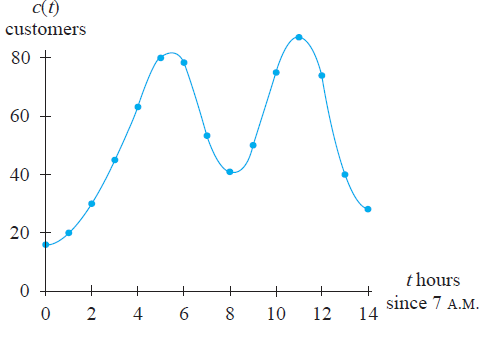
\includegraphics[scale = 1.5]{./img/sec23-1.png}
			\end{center}

			\begin{enumerate}[(a)]
				\item Estimate the average rate of change of the number of customers between 7am and 11am.  Interpret your answer.
					\vs{1}
					
				\item Estimate the instantaneous rate of change and percentage rate of change of the number of customers at 4pm.  Interpret your answers.
					\vs{1}
			\end{enumerate}			
		\end{ex}
	\clearpage
\end{document}